\documentclass{article}

\usepackage{amsmath}
\usepackage{amsfonts}
\usepackage{amssymb}
\usepackage{amsthm}
\usepackage{geometry}
\geometry{left=3cm, right=3cm, bottom=3cm, top=3cm}
\usepackage{tikz}
\usetikzlibrary{knots}

\newtheorem{proposition}{Proposition}
\newtheorem{lemma}{Lemma}
\newtheorem{theorem}{Theorem}
\theoremstyle{definition}
\newtheorem{example}{Example}


\begin{document}
\section{The Ribbon Disk Group}


As with a link group, the \textit{slice disk group} $\pi(S)$ of a slice disk $S$ in $D^4$ is the fundamental group of its complement in $D^4$. If the slice disk is in fact a ribbon $R$, then $\pi(R)$ is called its \textit{ribbon group}. We define the ribbon group of a ribbon in $S^3$ to be the ribbon group of its embedding into $D^4$ as in the proof of Theorem \ref{thm:ribbon-are-slice}. In this section, we are going to give an Wirtinger-like algorithm to compute ribbon groups.

To describe our procedure, we first need to establish some terminology. Let $R$ be a ribbon disk in $S^3$. A \textit{crossing} is a connected component of the set of ribbon singularities, i.e., the set of double points of the immersion $D^2 \rightarrow R$. Note that each crossing has a neighborhood as in Figure \ref{fig:nbhd-of-crossing-ribbon}. Denote by $J$ the set of singularities. Then a connected component of $R \setminus J$ will be called an \textit{arc} of $R$.

\begin{figure}[htb]
\centering
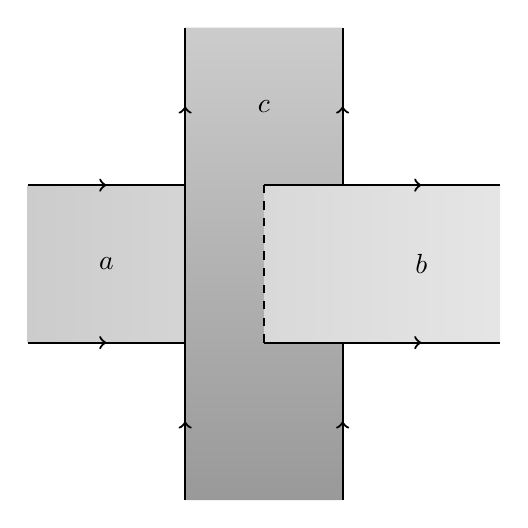
\begin{tikzpicture}
\clip (0, -2) rectangle (6, 4);
\shade[left color=black!20, right color = black!10] (0, 0) rectangle (6, 2);
\shade[bottom color=black!40, top color = black!20] (2, -2) -- (2, 4) -- (4, 4) -- (4, 2) -- (3, 2) -- (3, 0) -- (4, 0) -- (4, -2) -- (2, -2);
\draw[thick] (2, 0) -- (0, 0);
\draw[thick] (0, 2) -- (2, 2);
\draw[thick] (3, 2) -- (6, 2);
\draw[thick] (6, 0) -- (3, 0);
\draw[thick, dashed] (3, 0) -- (3, 2);
\draw[thick] (4, 2) -- (4, 4);
\draw[thick] (2, 4) -- (2, -2);
\draw[thick] (4, -2) -- (4, 0);

\draw[thick, ->] (0.9, 2) -- (1, 2);
\draw[thick, ->] (0.9, 0) -- (1, 0);

\draw[thick, ->] (4.9, 2) -- (5, 2);
\draw[thick, ->] (4.9, 0) -- (5, 0);

\draw[thick, ->] (2, -1.1) -- (2, -1);
\draw[thick, ->] (2, 2.9) -- (2, 3);
\draw[thick, ->] (4, -1.1) -- (4, -1);
\draw[thick, ->] (4, 2.9) -- (4, 3);


\node at (1, 1) {$a$};
\node at (5, 1) {$b$};
\node at (3, 3) {$c$};
\end{tikzpicture}
\caption{A neighborhood of a crossing with over-arc $c$ and under-arcs $a$ and $b$}
\label{fig:nbhd-of-crossing-ribbon}
\end{figure}

We are now ready to describe the desired procedure, henceforth referred to as the \textit{Ribbon Wirtinger procedure}. Let $S$ be in bijection with the set of arcs of~$R$. Now to any crossing as in Figure \ref{fig:nbhd-of-crossing-ribbon} assign a relation $bc = ca$. Then the presentation arising from this construction is a presentation of the ribbon group, as we will later show.


\begin{figure}[htb]
\centering
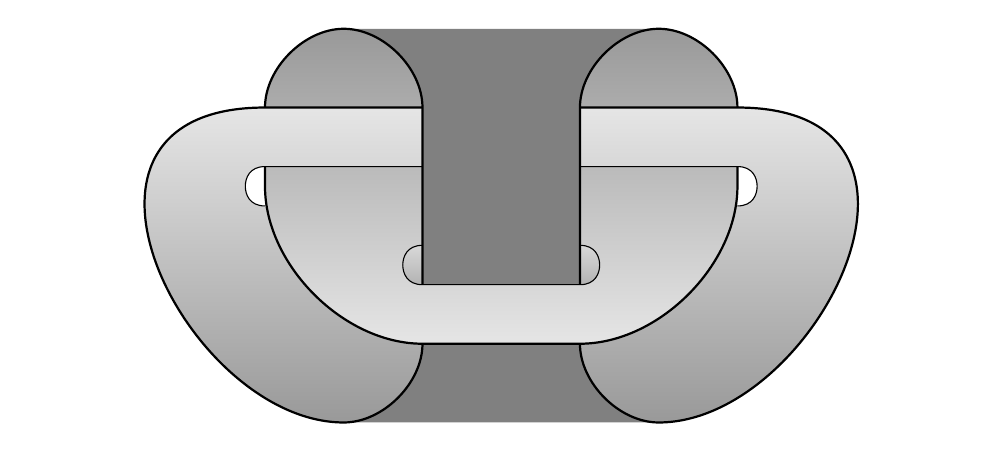
\begin{tikzpicture}
\fill[%pattern = north west lines
		color = black!50]
	(-2, 5) -- 
	(2, 5) .. controls +(-0.5, 0) and +(0, 0.5) ..
	(1, 4) -- 
	(1, 1) .. controls +(0, -0.5) and +(-0.5, 0) ..
	(2, 0) --
	(-2, 0) .. controls +(0.5, 0) and +(0, -0.5) ..
	(-1, 1) --
	(-1, 4) .. controls +(0, 0.5) and +(0.5, 0) ..
	(-2, 5);
	
\fill[top color = black!40, bottom color = black!10] 
	(-2, 5) .. controls +(-0.5, 0) and +(0, 0.5) ..
	(-3, 4) --
	(-3, 3) .. controls +(0, -1) and +(-1, 0) ..
	(-1, 1) -- 
	(1, 1) .. controls +(1, 0) and +(0, -1) ..
	(3, 3) -- 
	(3, 4) .. controls +(0, 0.5) and +(0.5, 0) ..
	(2, 5) .. controls +(-0.5, 0) and +(0, 0.5) ..
	(1, 4) --
	(1, 1.75) --
	(-1, 1.75) --
	(-1, 4) .. controls +(0, 0.5) and +(0.5, 0) ..
	(-2, 5);
	
\fill[bottom color = black!40, top color = black!10]
	(2, 0) .. controls +(2, 0) and +(3, 0) ..
	(3, 4) -- 
	(1, 4) --
	(1, 3.25) --
	(3, 3.25) --
	(3, 3) .. controls +(0, -1) and +(1, 0) ..
	(1, 1) .. controls +(0, -0.5) and +(-0.5, 0) ..
	(2, 0);
	
\fill[bottom color = black!40, top color = black!10]
	(-2, 0) .. controls +(-2, 0) and +(-3, 0) ..
	(-3, 4) -- 
	(-1, 4) --
	(-1, 3.25) --
	(-3, 3.25) --
	(-3, 3) .. controls +(0, -1) and +(-1, 0) ..
	(-1, 1) .. controls +(0, -0.5) and +(0.5, 0) ..
	(-2, 0);

\fill[bottom color=black!30, top color=black!15] 
	(-1, 2.25) .. controls +(-0.2, 0) and +(0, 0.1) ..
	(-1.25, 2) .. controls +(0, -0.1) and +(-0.2, 0) ..
	(-1, 1.75) -- (-1, 2.25);
\fill[bottom color=black!30, top color=black!15]
	(1, 1.75) .. controls +(0.2, 0) and +(0, -0.1) ..
	(1.25, 2) .. controls +(0, 0.1) and +(0.2, 0) ..
	(1, 2.25) -- (1, 1.75);	
	
\fill[color=white]
	(-3, 3.25) .. controls +(-0.2, 0) and +(0, 0.1) ..
	(-3.25, 3) .. controls +(0, -0.1) and +(-0.2, 0) ..
	(-3, 2.75);
\fill[color=white]
	(3, 3.25) .. controls +(0.2, 0) and +(0, 0.1) ..
	(3.25, 3) .. controls +(0, -0.1) and +(0.2, 0) ..
	(3, 2.75);
	
\draw (-1, 2.25) .. controls +(-0.2, 0) and +(0, 0.1) ..
	(-1.25, 2) .. controls +(0, -0.1) and +(-0.2, 0) ..
	(-1, 1.75) -- 
	(1, 1.75) .. controls +(0.2, 0) and +(0, -0.1) ..
	(1.25, 2) .. controls +(0, 0.1) and +(0.2, 0) ..
	(1, 2.25);

\draw (-1, 3.25) -- 
	(-3, 3.25) .. controls +(-0.2, 0) and +(0, 0.1) ..
	(-3.25, 3) .. controls +(0, -0.1) and +(-0.2, 0) ..
	(-3, 2.75);
\draw (1, 3.25) -- 
	(3, 3.25) .. controls +(0.2, 0) and +(0, 0.1) ..
	(3.25, 3) .. controls +(0, -0.1) and +(0.2, 0) ..
	(3, 2.75);
	
\draw[thick] (1, 1) .. controls +(0, -0.5) and +(-0.5, 0) ..
	(2, 0) .. controls +(2, 0) and +(3, 0) ..
	(3, 4) --
	(1, 4);
	
\draw[thick] (-1, 1) .. controls +(0, -0.5) and +(0.5, 0) ..
	(-2, 0) .. controls +(-2, 0) and +(-3, 0) ..
	(-3, 4) --
	(-1, 4);
	
\draw[thick] (-3, 3.25) -- (-3, 3) .. controls +(0, -1) and +(-1, 0) ..
	(-1, 1) -- 
	(1, 1)  .. controls +(1, 0) and +(0, -1) ..
	(3, 3) -- (3, 3.25);
	
\draw[thick] (-3, 4) .. controls +(0, 0.5) and +(-0.5, 0) ..
	(-2, 5) .. controls +(0.5, 0) and +(0, 0.5) ..
	(-1, 4) --
	(-1, 1.75);
	
\draw[thick] (3, 4) .. controls +(0, 0.5) and +(0.5, 0) ..
	(2, 5) .. controls +(-0.5, 0) and +(0, 0.5) ..
	(1, 4) --
	(1, 1.75);
\end{tikzpicture}
\caption{A ribbon disk without neighborhoods of the slits}
\label{fig:ribbon-nbhds-of-slits-removed}
\end{figure}


To prove that the above algorithm indeed gives rise to a presentation of the ribbon group, we will first need to address another (more complicated) procedure based on a Seifert-van Kampen argument not unlike the one we used in the proof of Theorem \ref{thm:wirtinger-thm}. First, we consider the embedding of $R$ into $D^4$ as in the proof of Theorem \ref{thm:ribbon-are-slice}. Let $P$ be the three-sphere in $D^4$ at the height of the inner (medium-gray) disk in Figure \ref{fig:ribbon-knots-are-slice}. Note that $P$ basically contains $R$, except for a neighborhood of the boundary of $R$ and for neighborhoods of slits, see Figure \ref{fig:ribbon-nbhds-of-slits-removed}. Now $P$ divides $D^4$ into two connected components. Let $H^+$ be the closure of the outer component and $H^-$ the closure of the inner component. The intersection of $R$ with a height in $H^+$, $P$ and $H^{-}$, respectively, is depicted in Figure \ref{fig:embedding-height-levels}.

\begin{figure}[htb]
\centering
\begin{minipage}{0.5\textwidth}
\centering
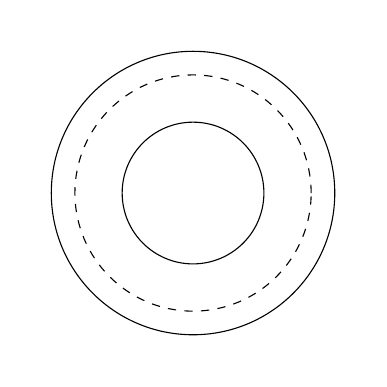
\begin{tikzpicture}[scale=0.6]
\clip (0, 0) circle (3.5);
\draw (0, 0) circle (3);
\draw (0, 0) circle (1.5);

\draw[dashed] (0, 0) circle (2.5);
\end{tikzpicture}
\end{minipage}%
\begin{minipage}{0.5\textwidth}
\centering
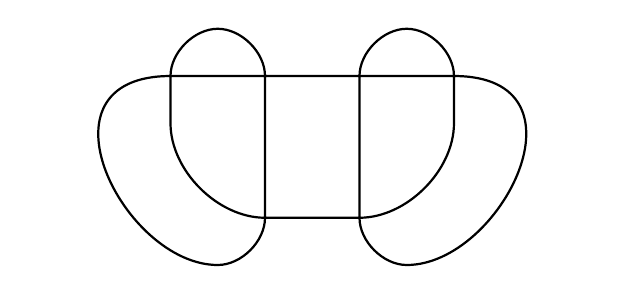
\begin{tikzpicture}[scale=0.6]
%\clip (-4, -2) rectangle (4, 5);
\begin{knot}[clip width = 5, consider self intersections = true, 
ignore endpoint intersections=false,
%draft mode = crossings,
flip crossing/.list = {4, 15, 9}
]
\draw[thick] (2, 0) .. controls +(2, 0) and +(3, 0) ..
	(3, 4) --
	(-3, 4) .. controls +(-3, 0) and +(-2, 0) ..
	(-2, 0) .. controls +(0.5, 0) and +(0, -0.5) ..
	(-1, 1) -- 
	(-1, 4) .. controls +(0, 0.5) and +(0.5, 0) ..
	(-2, 5) .. controls +(-0.5, 0) and +(0, 0.5) ..
	(-3, 4) --
	(-3, 3) .. controls +(0, -1) and +(-1, 0) ..
	(-1, 1) -- 
	(1, 1) .. controls +(1, 0) and +(0, -1) ..
	(3, 3) --
	(3, 4) .. controls +(0, 0.5) and +(0.5, 0) ..
	(2, 5) .. controls +(-0.5, 0) and +(0, 0.5) ..
	(1, 4) -- 
	(1, 1) .. controls +(0, -0.5) and +(-0.5, 0) ..
	(2, 0);
\end{knot}
\end{tikzpicture}
\end{minipage}

\begin{minipage}{0.5\textwidth}
\centering
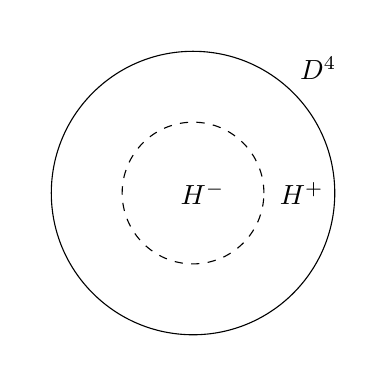
\begin{tikzpicture}[scale=0.6]
\clip (-3.5, -3.5) rectangle (3.5,3.5);
\draw (0, 0) circle (3);

\draw[dashed] (0, 0) circle (1.5);


\node at (0.2, 0) {$H^-$};
\node at (2.3, 0) {$H^+$};
\node at (2.65, 2.65) {$D^4$};

\end{tikzpicture}
\end{minipage}%
\begin{minipage}{0.5\textwidth}
\centering
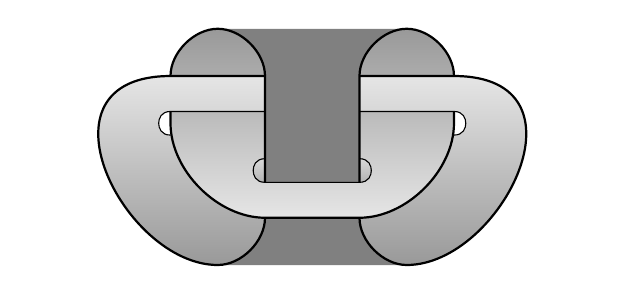
\begin{tikzpicture}[scale=0.6]
\fill[%pattern = north west lines
		color = black!50]
	(-2, 5) -- 
	(2, 5) .. controls +(-0.5, 0) and +(0, 0.5) ..
	(1, 4) -- 
	(1, 1) .. controls +(0, -0.5) and +(-0.5, 0) ..
	(2, 0) --
	(-2, 0) .. controls +(0.5, 0) and +(0, -0.5) ..
	(-1, 1) --
	(-1, 4) .. controls +(0, 0.5) and +(0.5, 0) ..
	(-2, 5);
	
\fill[top color = black!40, bottom color = black!10] 
	(-2, 5) .. controls +(-0.5, 0) and +(0, 0.5) ..
	(-3, 4) --
	(-3, 3) .. controls +(0, -1) and +(-1, 0) ..
	(-1, 1) -- 
	(1, 1) .. controls +(1, 0) and +(0, -1) ..
	(3, 3) -- 
	(3, 4) .. controls +(0, 0.5) and +(0.5, 0) ..
	(2, 5) .. controls +(-0.5, 0) and +(0, 0.5) ..
	(1, 4) --
	(1, 1.75) --
	(-1, 1.75) --
	(-1, 4) .. controls +(0, 0.5) and +(0.5, 0) ..
	(-2, 5);
	
\fill[bottom color = black!40, top color = black!10]
	(2, 0) .. controls +(2, 0) and +(3, 0) ..
	(3, 4) -- 
	(1, 4) --
	(1, 3.25) --
	(3, 3.25) --
	(3, 3) .. controls +(0, -1) and +(1, 0) ..
	(1, 1) .. controls +(0, -0.5) and +(-0.5, 0) ..
	(2, 0);
	
\fill[bottom color = black!40, top color = black!10]
	(-2, 0) .. controls +(-2, 0) and +(-3, 0) ..
	(-3, 4) -- 
	(-1, 4) --
	(-1, 3.25) --
	(-3, 3.25) --
	(-3, 3) .. controls +(0, -1) and +(-1, 0) ..
	(-1, 1) .. controls +(0, -0.5) and +(0.5, 0) ..
	(-2, 0);

\fill[bottom color=black!30, top color=black!15] 
	(-1, 2.25) .. controls +(-0.2, 0) and +(0, 0.1) ..
	(-1.25, 2) .. controls +(0, -0.1) and +(-0.2, 0) ..
	(-1, 1.75) -- (-1, 2.25);
\fill[bottom color=black!30, top color=black!15]
	(1, 1.75) .. controls +(0.2, 0) and +(0, -0.1) ..
	(1.25, 2) .. controls +(0, 0.1) and +(0.2, 0) ..
	(1, 2.25) -- (1, 1.75);	
	
\fill[color=white]
	(-3, 3.25) .. controls +(-0.2, 0) and +(0, 0.1) ..
	(-3.25, 3) .. controls +(0, -0.1) and +(-0.2, 0) ..
	(-3, 2.75);
\fill[color=white]
	(3, 3.25) .. controls +(0.2, 0) and +(0, 0.1) ..
	(3.25, 3) .. controls +(0, -0.1) and +(0.2, 0) ..
	(3, 2.75);
	
\draw (-1, 2.25) .. controls +(-0.2, 0) and +(0, 0.1) ..
	(-1.25, 2) .. controls +(0, -0.1) and +(-0.2, 0) ..
	(-1, 1.75) -- 
	(1, 1.75) .. controls +(0.2, 0) and +(0, -0.1) ..
	(1.25, 2) .. controls +(0, 0.1) and +(0.2, 0) ..
	(1, 2.25);

\draw (-1, 3.25) -- 
	(-3, 3.25) .. controls +(-0.2, 0) and +(0, 0.1) ..
	(-3.25, 3) .. controls +(0, -0.1) and +(-0.2, 0) ..
	(-3, 2.75);
\draw (1, 3.25) -- 
	(3, 3.25) .. controls +(0.2, 0) and +(0, 0.1) ..
	(3.25, 3) .. controls +(0, -0.1) and +(0.2, 0) ..
	(3, 2.75);
	
\draw[thick] (1, 1) .. controls +(0, -0.5) and +(-0.5, 0) ..
	(2, 0) .. controls +(2, 0) and +(3, 0) ..
	(3, 4) --
	(1, 4);
	
\draw[thick] (-1, 1) .. controls +(0, -0.5) and +(0.5, 0) ..
	(-2, 0) .. controls +(-2, 0) and +(-3, 0) ..
	(-3, 4) --
	(-1, 4);
	
\draw[thick] (-3, 3.25) -- (-3, 3) .. controls +(0, -1) and +(-1, 0) ..
	(-1, 1) -- 
	(1, 1)  .. controls +(1, 0) and +(0, -1) ..
	(3, 3) -- (3, 3.25);
	
\draw[thick] (-3, 4) .. controls +(0, 0.5) and +(-0.5, 0) ..
	(-2, 5) .. controls +(0.5, 0) and +(0, 0.5) ..
	(-1, 4) --
	(-1, 1.75);
	
\draw[thick] (3, 4) .. controls +(0, 0.5) and +(0.5, 0) ..
	(2, 5) .. controls +(-0.5, 0) and +(0, 0.5) ..
	(1, 4) --
	(1, 1.75);
\end{tikzpicture}
\end{minipage}

\begin{minipage}{0.5\textwidth}
\centering
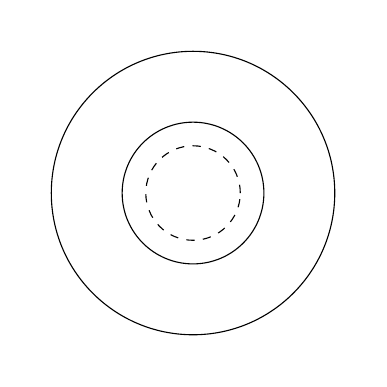
\begin{tikzpicture}[scale=0.6]
\clip (0, 0) circle (3.5);
\draw (0, 0) circle (3);
\draw (0, 0) circle (1.5);

\draw[dashed] (0, 0) circle (1);

\end{tikzpicture}
\end{minipage}%
\begin{minipage}{0.5\textwidth}
\centering
\begin{tikzpicture}[scale=0.6]
\clip (-3, 0) rectangle (3, 5);
\draw (-1, 2.25) .. controls +(-0.2, 0) and +(0, 0.1) ..
	(-1.25, 2) .. controls +(0, -0.1) and +(-0.2, 0) ..
	(-1, 1.75) -- (1, 1.75) 
	.. controls +(0.2, 0) and +(0, -0.1) .. (1.25, 2)
	.. controls +(0, 0.1) and +(0.2, 0) .. (1, 2.25)
	-- (-1, 2.25);
	
\draw (-2, 3.25) .. controls +(-0.2, 0) and +(0, 0.1) ..
	(-2.25, 3) .. controls +(0, -0.1) and +(-0.2, 0) ..
	(-2, 2.75) -- (2, 2.75) 
	.. controls +(0.2, 0) and +(0, -0.1) .. (2.25, 3)
	.. controls +(0, 0.1) and +(0.2, 0) .. (2, 3.25)
	-- (-2, 3.25);



\end{tikzpicture}
\end{minipage}
\caption{The embedding of $R$ (right) into $D^4$ (left) at different heights}
\label{fig:embedding-height-levels}
\end{figure}

We are now going to apply the Seifert-van Kampen Theorem to the decomposition 
$$D^4 \setminus R = (H^+ \setminus R) \cup (H^- \setminus R).$$ From Figure \ref{fig:embedding-height-levels} it is evident that the interior of $H^+$ retracts onto $S^3 \setminus \partial R$, so we get an isomorphism $\pi_1(H^+ \setminus R) \cong \pi(K)$. Similarly, $\pi_1(H^- \setminus R)$ is a free group generated by meridians of $K$. One immediate consequence of this is the following.

\begin{proposition}
Let $R$ be a ribbon disk for a knot $K$. Then $\pi(R)$ is a quotient of $\pi(K)$.
\end{proposition}

\begin{proof}
Any generator of $\pi_1(H^- \setminus R)$ is represented by a meridian in $\pi_1(H^+ \setminus R)$. Thus, by the Seifert-van Kampen Theorem, $\pi(R)$ is isomorphic to a quotient of $\pi_1(H^+ \setminus R)$.
\end{proof}

We are now going to work towards a more concrete description of $\pi(R)$ by inspecting the space $P \setminus R$, see Figure \ref{fig:ribbon-nbhds-of-slits-removed}. Let us first consider two meridians in $P \setminus R$ that pass through the same hole. Then, assuming they are coherently oriented, there is a homotopy between said curves in $H^- \setminus R$. This yields a set of relations, referred to as the \textit{same-slit-relations}, identifying meridians in $\pi(K)$ passing through the same slit in $P \setminus R$. An example pair of meridians identified by the same-slit-relations is depicted in Figure \ref{fig:same-slit}.

\begin{figure}[htb]
\centering
\begin{minipage}[b]{0.6\textwidth}
\centering
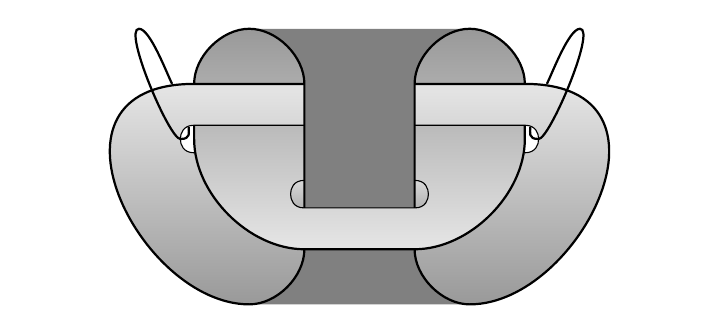
\begin{tikzpicture}[scale=0.7]

\fill[%pattern = north west lines
		color = black!50]
	(-2, 5) -- 
	(2, 5) .. controls +(-0.5, 0) and +(0, 0.5) ..
	(1, 4) -- 
	(1, 1) .. controls +(0, -0.5) and +(-0.5, 0) ..
	(2, 0) --
	(-2, 0) .. controls +(0.5, 0) and +(0, -0.5) ..
	(-1, 1) --
	(-1, 4) .. controls +(0, 0.5) and +(0.5, 0) ..
	(-2, 5);
	
\fill[top color = black!40, bottom color = black!10] 
	(-2, 5) .. controls +(-0.5, 0) and +(0, 0.5) ..
	(-3, 4) --
	(-3, 3) .. controls +(0, -1) and +(-1, 0) ..
	(-1, 1) -- 
	(1, 1) .. controls +(1, 0) and +(0, -1) ..
	(3, 3) -- 
	(3, 4) .. controls +(0, 0.5) and +(0.5, 0) ..
	(2, 5) .. controls +(-0.5, 0) and +(0, 0.5) ..
	(1, 4) --
	(1, 1.75) --
	(-1, 1.75) --
	(-1, 4) .. controls +(0, 0.5) and +(0.5, 0) ..
	(-2, 5);
	
\fill[bottom color = black!40, top color = black!10]
	(2, 0) .. controls +(2, 0) and +(3, 0) ..
	(3, 4) -- 
	(1, 4) --
	(1, 3.25) --
	(3, 3.25) --
	(3, 3) .. controls +(0, -1) and +(1, 0) ..
	(1, 1) .. controls +(0, -0.5) and +(-0.5, 0) ..
	(2, 0);
	
\fill[bottom color = black!40, top color = black!10]
	(-2, 0) .. controls +(-2, 0) and +(-3, 0) ..
	(-3, 4) -- 
	(-1, 4) --
	(-1, 3.25) --
	(-3, 3.25) --
	(-3, 3) .. controls +(0, -1) and +(-1, 0) ..
	(-1, 1) .. controls +(0, -0.5) and +(0.5, 0) ..
	(-2, 0);

\fill[bottom color=black!30, top color=black!15] 
	(-1, 2.25) .. controls +(-0.2, 0) and +(0, 0.1) ..
	(-1.25, 2) .. controls +(0, -0.1) and +(-0.2, 0) ..
	(-1, 1.75) -- (-1, 2.25);
\fill[bottom color=black!30, top color=black!15]
	(1, 1.75) .. controls +(0.2, 0) and +(0, -0.1) ..
	(1.25, 2) .. controls +(0, 0.1) and +(0.2, 0) ..
	(1, 2.25) -- (1, 1.75);	
	
	
	
\fill[color=white]
	(-3, 3.25) .. controls +(-0.2, 0) and +(0, 0.1) ..
	(-3.25, 3) .. controls +(0, -0.1) and +(-0.2, 0) ..
	(-3, 2.75);
\fill[color=white]
	(3, 3.25) .. controls +(0.2, 0) and +(0, 0.1) ..
	(3.25, 3) .. controls +(0, -0.1) and +(0.2, 0) ..
	(3, 2.75);
	

%meridians start
\draw[thick]
	 (-3.1, 3.22) .. controls +(0, -0.1) and +(0.2, 0) ..
	 (-3.25, 3) .. controls +(-0.2, 0) and +(-0.3, 0) ..
	 (-4, 5) .. controls +(0.2, 0) and +(-0.1, 0.2) ..
	 (-3.4, 4);
	
\draw[thick]
	 (3.1, 3.22) .. controls +(0, -0.1) and +(-0.2, 0) ..
	 (3.25, 3) .. controls +(0.2, 0) and +(0.3, 0) ..
	 (4, 5) .. controls +(-0.2, 0) and +(0.1, 0.2) ..
	 (3.4, 4);
%meridians end
	 
	
\draw (-1, 2.25) .. controls +(-0.2, 0) and +(0, 0.1) ..
	(-1.25, 2) .. controls +(0, -0.1) and +(-0.2, 0) ..
	(-1, 1.75) -- 
	(1, 1.75) .. controls +(0.2, 0) and +(0, -0.1) ..
	(1.25, 2) .. controls +(0, 0.1) and +(0.2, 0) ..
	(1, 2.25);

\draw (-1, 3.25) -- 
	(-3, 3.25) .. controls +(-0.2, 0) and +(0, 0.1) ..
	(-3.25, 3) .. controls +(0, -0.1) and +(-0.2, 0) ..
	(-3, 2.75);
\draw (1, 3.25) -- 
	(3, 3.25) .. controls +(0.2, 0) and +(0, 0.1) ..
	(3.25, 3) .. controls +(0, -0.1) and +(0.2, 0) ..
	(3, 2.75);
	
\draw[thick] (1, 1) .. controls +(0, -0.5) and +(-0.5, 0) ..
	(2, 0) .. controls +(2, 0) and +(3, 0) ..
	(3, 4) --
	(1, 4);
	
\draw[thick] (-1, 1) .. controls +(0, -0.5) and +(0.5, 0) ..
	(-2, 0) .. controls +(-2, 0) and +(-3, 0) ..
	(-3, 4) --
	(-1, 4);
	
\draw[thick] (-3, 3.25) -- (-3, 3) .. controls +(0, -1) and +(-1, 0) ..
	(-1, 1) -- 
	(1, 1)  .. controls +(1, 0) and +(0, -1) ..
	(3, 3) -- (3, 3.25);
	
\draw[thick] (-3, 4) .. controls +(0, 0.5) and +(-0.5, 0) ..
	(-2, 5) .. controls +(0.5, 0) and +(0, 0.5) ..
	(-1, 4) --
	(-1, 1.75);
	
\draw[thick] (3, 4) .. controls +(0, 0.5) and +(0.5, 0) ..
	(2, 5) .. controls +(-0.5, 0) and +(0, 0.5) ..
	(1, 4) --
	(1, 1.75);


\end{tikzpicture}
\caption{Same-slit-relations}
\label{fig:same-slit}
\end{minipage}%
\begin{minipage}[b]{0.4\textwidth}
\centering
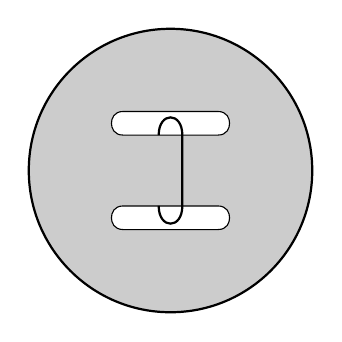
\begin{tikzpicture}[scale=0.6]
\fill[color = black!20] (0, 0) circle (3);
\draw[thick] (0, 0) circle (3);
\draw[fill = white] 
	(-1.25, -1) .. controls +(0, 0.1) and +(-0.2, 0) ..
	(-1, -0.75) --
	(1, -0.75) .. controls +(0.2, 0) and +(0, 0.1) ..
	(1.25, -1) .. controls +(0, -0.1) and +(0.2, 0) ..
	(1, -1.25) --
	(-1, -1.25) .. controls +(-0.2, 0) and +(0, -0.1) ..
	(-1.25, -1);
\draw[fill = white] 
	(-1.25, 1) .. controls +(0, -0.1) and +(-0.2, 0) ..
	(-1, 0.75) --
	(1, 0.75) .. controls +(0.2, 0) and +(0, -0.1) ..
	(1.25, 1) .. controls +(0, 0.1) and +(0.2, 0) ..
	(1, 1.25) --
	(-1, 1.25) .. controls +(-0.2, 0) and +(0, 0.1) ..
	(-1.25, 1);
\draw[thick] 
	(-0.25, -0.75) .. controls +(0, -0.5) and +(0, -0.5) ..
	(0.25, -0.75) --
	(0.25, 0.75) .. controls +(0, 0.5) and +(0, 0.5) ..
	(-0.25, 0.75);
\end{tikzpicture}
\caption{Through-slit-relations}
\label{fig:an-interesting-curve}
\end{minipage}
\end{figure}

The final set of relations is a little bit more subtle to see. Note that $\pi_1(P \setminus R)$ is not generated by meridians as previously discussed. In addition, we need to consider curves nullhomotopic in $H^+ \setminus P$ that pass through slits. Including such curves into $\pi_1(H^- \setminus R)$ gives rise to the so-called \textit{through-slit-relations}. A toy example can be found in Figure \ref{fig:an-interesting-curve}. We can now summarize our procedure as follows.

\begin{lemma}
Let $R$ be a ribbon disk for $K$.
A presentation of $\pi(R)$ can be obtained by adding same-slit-relations and through-slit-relations to a presentation of $\pi(K)$.
\end{lemma}

\begin{figure}[htb]
\centering
\begin{minipage}{0.5\textwidth}
\centering

\begin{tikzpicture}
\clip (0, 0) rectangle (5, 2.75);
\fill[left color=black!10, right color=black!30] (0, 0) rectangle (5, 2);
\draw[thick] (0, 0) -- (5, 0);
\draw[thick] (0, 2) -- (5, 2);
\end{tikzpicture}
\end{minipage}%
\begin{minipage}{0.5\textwidth}
\centering
\begin{tikzpicture}
\begin{knot}[clip width = 5, ignore endpoint intersections=false, flip crossing = 1]
\strand[thick] (0, 0) -- (5, 0);
\strand[thick] (0, 2) -- (5, 2);
\strand[thick] (2.5, 2) ellipse (0.3 and 0.75);
\end{knot}
\end{tikzpicture}
\end{minipage}
\caption{Interpretation of the arcs in the Ribbon Wirtinger procedure}
\label{fig:arcs-interpretation}
\end{figure}


\begin{theorem}
The Ribbon Wirtinger procedure is correct.
\end{theorem}

\begin{proof}
The main ingredient used to check correctness is interpreting the generating set of the Ribbon Wirtinger procedure as meridians such as the meridian in Figure \ref{fig:arcs-interpretation}. It is then immediate that the through-slit relations, the same-slit relations and the Wirtinger relations are all satisfied. The converse is also true.
\end{proof}

\end{document}
